\documentclass[11pt]{article}

\usepackage[margin=0.5in]{geometry}
\usepackage{amsmath, amssymb}
\usepackage{graphicx}
\usepackage{hyperref}
\usepackage{xcolor}
\usepackage{booktabs}
\usepackage{titlesec}

\titlespacing*{\section}{0pt}{4pt}{2pt}
\titlespacing*{\subsection}{0pt}{3pt}{1.5pt}
\titlespacing*{\subsubsection}{0pt}{2pt}{1pt}

\newcommand{\code}[1]{%
    \colorbox{gray!40}{\texttt{#1}}%
}

\setlength{\abovedisplayskip}{4pt}
\setlength{\belowdisplayskip}{4pt}
\setlength{\parskip}{1.5pt}

\makeatletter
\renewcommand\@listI{\leftmargin\leftmargini
  \topsep=1.5pt \parsep=0pt \itemsep=0.5pt \partopsep=0pt}
\makeatother

\raggedbottom

\title{IRE Assignment Design Note}
\author{Iman Kalyan Chakraborty - 2026801003}
\date{\today}

\begin{document}

\maketitle

\section{Introduction}

This assignment implements a complete lexical and semantic retrieval pipeline for news
recommendation over two real-world datasets, EB-NeRD (demo, small, and large variants) and MIND
(small and large variants). The two datasets differ in language, storage schema, and scale. The
small and demo variants were used for experimentation; the large variants for the real Codabench
submissions.

\begin{sloppypar}
The pipeline has four stages: \textbf{unified schema conversion}, since the two datasets' raw
formats differ and must share one format before use; \textbf{lexical candidate generation} via a
from-scratch BM25 implementation, faster than the \code{rank\_bm25} package; \textbf{semantic
candidate generation} via \code{paraphrase-xlm-r-multilingual-v1} embeddings, multilingual since
EB-NeRD is Danish and MIND is English; and \textbf{evaluation} against every required metric:
AUC, MRR, nDCG@k, diversity, novelty, and coverage.
\end{sloppypar}

The rest of this report covers each stage's design decisions in Section~\ref{sec:design}, then
the resulting experimental findings in Section~\ref{sec:discussion}, including a real
large-scale engineering incident hit while running Q4 (Section~\ref{sec:incident}).

\section{Design}
\label{sec:design}

\subsection{Unified Schema}

EB-NeRD (Danish, Parquet, provider-supplied embeddings, no entities) and MIND (English, TSV, no
embeddings of its own, knowledge-graph entities) share almost nothing at the raw-file level. An
early choice was to convert both into one common schema and write every downstream stage (Q2
through Q5) against that schema only, not five dataset-specific code paths.

\begin{sloppypar}
Three tables cover both. \textbf{articles} holds \code{article\_id}, \code{title},
\code{abstract}, \code{body}, \code{category}, \code{published\_time}, \code{dataset}.
\textbf{behaviors} holds one row per impression: \code{impression\_id}, \code{user\_id},
\code{impression\_time}, \code{article\_ids\_inview}, \code{article\_ids\_clicked},
\code{session\_id}, \code{split}, \code{dataset}. \textbf{history} holds each user's pre-window
click sequence: \code{article\_id\_sequence}, \code{timestamp\_sequence},
\code{read\_time\_sequence}, \code{scroll\_percentage\_sequence}. A column only one raw format
actually has is left null or absent rather than fabricated: MIND parses no \code{body} text, and
the real, blind \code{ebnerd\_testset} has no \code{article\_ids\_clicked}. A placeholder was
considered and rejected, since it would hide exactly the cases where the absence itself is the
load-bearing fact.

The datasets are never merged despite sharing a schema: each builds into its own output
directory, and every ID is namespaced (\code{ebnerd\_123}, \code{mind\_N55528}), so a bug can
never silently join rows across them. This also enforces Q9's anti-gaming requirement at the
schema level, not as an afterthought: EB-NeRD's raw behaviors carry look-ahead fields,
\code{next\_read\_time} and \code{next\_scroll\_percentage}, that would leak future engagement if
used as features. The unified schema simply never carries them, and a test,
\code{test\_no\_leakage\_columns}, asserts this against the real on-disk schema every run.
\end{sloppypar}

\subsection{Q1: Reproducible Data Pipeline}

The split is never random. Each dataset's provider train split is followed by its provider
dev/validation split, in that time order. The provider's dev/validation split becomes the
held-out \textbf{test} set; \textbf{val} is carved from the last day of the provider
\textbf{train} split, by time. A random split was rejected: it would leak future articles and
trends into training.

Two leakage checks run at build time: EB-NeRD's history timestamps must precede every impression
for that user, and MIND's per-row history string must be identical across all of a user's rows,
confirming a fixed pre-window snapshot. The pipeline rebuilds from raw files with one command,
with a test cell after every step, so a broken build fails loudly instead of silently writing
wrong data.

\subsection{Q2: Lexical Candidate Generation (BM25)}

BM25 is implemented from scratch in \code{bm25.py} instead of \code{rank\_bm25}, purely for
speed. \code{rank\_bm25}'s plain per-term dictionary lookup measured near 3 seconds per query on
MIND's 65,238-article corpus, over 40 hours at the scale needed here. A real postings-list index,
scored with a vectorized numpy operation and \code{np.argpartition} for top-K, measured about
5ms per query instead, roughly a thousand times faster.

A user's query is their most recent 20 clicked titles, concatenated. Since this depends only on
a fixed history, the top-200 scores are computed once per user and cached; recall@50/100 are
read off as prefixes of that list instead of re-scoring. Recall@K is a fraction,
$|clicked \cap top\text{-}K| / |clicked|$, not a plain hit or miss, since one impression can
have more than one clicked article.

\subsection{Q3: Semantic Candidate Generation (Embeddings)}

One embedding model, \code{paraphrase-xlm-r-multilingual-v1}, is used for both datasets (not
EB-NeRD's own provided embeddings), so Danish and English text share one vector space. MIND has
no article embeddings of its own, only unrelated knowledge-graph entity vectors.

Embeddings are computed once on a Kaggle GPU notebook and saved as parquet, so the local
environment never installs \code{sentence-transformers}/\code{torch}. Retrieval is a
brute-force batched matrix multiply plus \code{argpartition}, not FAISS: at this corpus size (up
to about 65,000 articles), the full MIND val/test population retrieves in well under two
minutes, batched in groups of a few thousand users since the full similarity matrix would
otherwise take roughly 17GB at once.

A user's representation is the mean of their last 20 clicked embeddings, the same window Q2
uses, so Section~\ref{sec:lexvssem}'s comparison only varies the method.

\subsection{Q4: Offline Evaluation Harness}

AUC, MRR, and nDCG need a full ranking over candidates with known labels. The only such set per
impression is \code{article\_ids\_inview} (what the user was shown), not the whole catalog. This
differs from Q2/Q3's recall@K, which asks whether a method can find the clicked article at all;
here the question is whether it ranks the clicked article near the top among what was shown. Q4
cannot reuse Q2/Q3's saved top-200 lists for this, since MIND's recall@200 is only a few percent
and the clicked article is usually not in it. Instead a re-scoring adapter, \code{score\_inview},
scores each method for exactly one impression's inview set, on the fly.

Beyond-accuracy: intra-list diversity is one minus the average same-category-pair share in the
top-10 list; novelty is the negative log of an item's train-click share (add-one smoothed);
coverage is the catalog fraction appearing in the saved top-200 lists (computed once per dataset,
not per split). Cold-start vs. warm is the required slice; head vs. tail (top 20\% by train
clicks vs. the rest) is a second. Every metric carries a 95\% bootstrap CI over 1,000 resamples.

\subsection{Q5: Codabench Submission}
\label{sec:q5}

The submission format, one line per impression as
\code{\{impression\_id\} [rank\_1,...,rank\_n]} in the original row order, was confirmed
directly from MIND's Submission Guidelines page and matches both the EB-NeRD starter
repository and the reference MIND example code. Prediction files were generated for all three
dataset tracks with \code{generate\_predictions.py}, reusing Q4's \code{score\_inview}
adapters.

\begin{sloppypar}
The Codabench competitions grade against a separate, hidden test population
(\code{MINDlarge\_test}, \code{ebnerd\_testset.zip}), not the local provider dev/validation
\texttt{test} split. MIND's 26{,}228 test-only articles (of 120{,}961) are re-encoded on a fresh
Kaggle GPU pass; the rest reuse existing embeddings. EB-NeRD needs no new embeddings, since its
test catalog was verified byte-for-byte identical to \code{ebnerd\_large}'s. Both wrote valid,
round-trip-tested prediction zips (2{,}370{,}727 and 13{,}336{,}710 lines, matching each
population's impression count exactly), submitting \code{embedding} per its Q4-measured edge
(Section~\ref{sec:lexvssem}).
\end{sloppypar}

\subsubsection*{Leaderboard Screenshots}

MIND: both methods scored on the real \code{MINDlarge\_test} leaderboard.
\code{embedding} reaches AUC 0.6174 (rank 55); \code{bm25} reaches AUC 0.5797.

\begin{center}
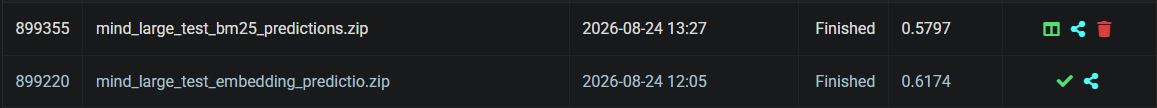
\includegraphics[width=0.46\textwidth]{mind_results.png}\\[1pt]
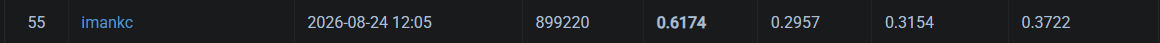
\includegraphics[width=0.46\textwidth]{mind_leaderboard_rank.png}
\end{center}

EB-NeRD: Codabench's own evaluation queue was still processing the submission at writing time
(server-side scoring time, not under this pipeline's control). The screenshot shows the
submission accepted and queued, not yet a scored row; it will be updated once Codabench returns
a score. The cancelled ones were cancelled after $\sim$4-5 hours of processing.

\begin{center}
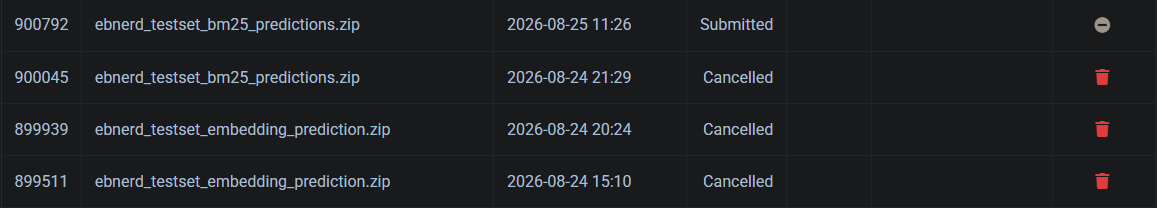
\includegraphics[width=0.62\textwidth]{ebnerd_results.png}
\end{center}

\subsection{Code Optimizations}
\label{sec:codeopt}

Several real performance and memory problems were found and fixed while running the pipeline at
full scale, in the order encountered.

\begin{sloppypar}
\small
\setlength{\itemsep}{1pt}
\begin{itemize}
\item \textbf{\code{rank\_bm25}'s per-term lookup was the Q2 bottleneck}: near 3 seconds per
query, over 40 hours at the scale needed. A postings-list index with vectorized numpy and
\code{argpartition} top-K cut this to about 5ms per query, roughly 1000$\times$ faster.

\item \textbf{Pandas hit a memory and throughput ceiling at \code{ebnerd\_large}/\code{mind\_large}
scale}. The full pipeline was rewritten to polars (lazy scans, columnar operations), which made
large-dataset runs tractable at all.

\item \textbf{Writing Q2/Q3's dense top-K list column in one shot ran out of memory, and
\code{gc.collect()} cost minutes per call against large notebook state}. A chunked write merged
with \code{pyarrow.ParquetWriter} bounded peak memory; \code{gc.collect()} was removed entirely,
since Python's own refcounting already frees the memory.

\item \textbf{Q3's \code{batched\_top\_k} results-list accumulation raised a \code{MemoryError} at
MIND scale}. Reducing \code{QUERY\_CHUNK\_SIZE}/\code{BATCH\_SIZE} fixed this with no functional
change.

\item \textbf{\code{cosine\_similarity\_subset} rebuilt a 125K-entry dictionary and renormalized
the corpus subset on every one of over 12.5 million calls (Q4/Q5)}. Precomputing
\code{id\_to\_idx}/\code{corpus\_unit} once per dataset turned an unfinished run (under 1/8 of
the passes done in 2h21m) into all four Q5 passes ($\sim$12.9M impressions) in $\sim$99 min.

\item \textbf{A dict per impression cost several GB of overhead at Q4's 12.5-million-impression
scale}. Preallocated numpy arrays per scalar column avoided this entirely.

\item \textbf{Both large datasets loaded together left under 0.3GB free RAM}: dead \code{train}
rows stayed resident, and \code{top10\_ids} grew linearly with rows scored. Loading one dataset
per kernel (\code{EVAL\_DATASETS}), dropping \code{train} rows after their stats are computed,
and canonicalizing IDs through a shared string pool freed about 42\% of \code{behaviors} and
made \code{mind\_large} crash-free.

\item \textbf{\code{WinError 10055} kernel crashes could lose a scoring pass or corrupt a
checkpoint mid-write}. Checkpointing every 200,000 rows, writing atomically via
\code{os.replace}, retrying automatically, and dropping a redundant \code{.astype(np.float32)}
copy meant a crash cost minutes rather than hours, and checkpoints were always valid.

\item \textbf{Bootstrap CI over 28.5 million rows still crashed inside Jupyter even fully
checkpointed}: filtering the whole \code{DataFrame} per slice also wasted more memory than
needed. A standalone script, with no Jupyter involved, finished the computation from the
checkpoints, filtering one metric column per slice at a time. \code{ebnerd\_large}'s Q4 finished
this way, with no crash.
\end{itemize}
\end{sloppypar}

\section{Discussion}
\label{sec:discussion}

\subsection{Results}
\label{sec:results}

Table \ref{tab:results} collects every core metric, recall@200, catalog coverage, AUC, and
nDCG@10, for both methods across every dataset track and split. Coverage is computed once per
dataset (not per split), so its value repeats across a dataset's two rows.

\begin{table}[h]
\centering
\scriptsize
\setlength{\tabcolsep}{3pt}
\renewcommand{\arraystretch}{0.95}
\begin{tabular}{ll cc cc cc cc}
\toprule
& & \multicolumn{2}{c}{Recall@200} & \multicolumn{2}{c}{Coverage} & \multicolumn{2}{c}{AUC} & \multicolumn{2}{c}{nDCG@10} \\
\cmidrule(lr){3-4} \cmidrule(lr){5-6} \cmidrule(lr){7-8} \cmidrule(lr){9-10}
Dataset & Split & BM25 & Emb & BM25 & Emb & BM25 & Emb & BM25 & Emb \\
\midrule
EB-NeRD demo & val & 3.51\% & 2.85\% & 92.0\% & 56.0\% & 0.504 & 0.569 & 0.445 & 0.483 \\
EB-NeRD demo & test & 2.85\% & 2.61\% & 92.0\% & 56.0\% & 0.500 & 0.553 & 0.433 & 0.465 \\
EB-NeRD small & val & 2.10\% & 1.48\% & 97.0\% & 71.5\% & 0.508 & 0.557 & 0.452 & 0.480 \\
EB-NeRD small & test & 1.82\% & 1.49\% & 97.0\% & 71.5\% & 0.501 & 0.550 & 0.434 & 0.464 \\
EB-NeRD large & val & 0.53\% & 0.29\% & 98.7\% & 77.8\% & 0.509 & 0.559 & 0.454 & 0.483 \\
EB-NeRD large & test & 0.63\% & 0.21\% & 98.7\% & 77.8\% & 0.501 & 0.552 & 0.435 & 0.465 \\
MIND small & val & 3.40\% & 2.39\% & 99.5\% & 96.7\% & 0.559 & 0.610 & 0.324 & 0.349 \\
MIND small & test & 1.61\% & 1.92\% & 99.5\% & 96.7\% & 0.556 & 0.595 & 0.336 & 0.361 \\
MIND large & val & 2.97\% & 1.99\% & 99.9\% & 99.1\% & 0.559 & 0.610 & 0.325 & 0.352 \\
MIND large & test & 1.32\% & 1.52\% & 99.9\% & 99.1\% & 0.557 & 0.594 & 0.338 & 0.361 \\
\bottomrule
\end{tabular}
\caption{\small Recall@200, catalog coverage, AUC, and nDCG@10 for lexical (BM25) vs. semantic
(embedding) candidate generation, across every dataset track and split. The \emph{large} rows
are the real Codabench-track catalogs (125,541/104,151 articles); recall@200 is naturally lower
there than on the smaller catalogs. AUC/nDCG@10 are Q4's offline metrics on the local
\texttt{test} split, distinct from Q5's real Codabench scores (Section~\ref{sec:q5}).}
\label{tab:results}
\end{table}

\subsection{Lexical vs. Semantic Retrieval}
\label{sec:lexvssem}

All numbers here were produced on one CPU-only machine (Intel Core i5-13500, 14 cores/20
threads, 16GB RAM); the pipeline's only GPU use is Q3's one-time Kaggle embedding computation
(Section~\ref{sec:design}). BM25 leads recall@200 (defined in Section~\ref{sec:design}'s Q2
subsection as the clicked-article fraction found in the top-200 retrieved list) almost
everywhere in Table \ref{tab:results}, except MIND's test split, where embeddings overtake it at
both recall@50 (0.65\% vs. 0.45\%) and recall@200. BM25 also covers more of each catalog:
coverage ranges 92.0--99.9\% for BM25 versus 56.0--99.1\% for embeddings, since mean-pooled
vectors concentrate retrieval on a narrower slice.

This reverses under Q4's AUC, scored only on the small inview set shown to a user. At both real
Codabench scales, MIND large's test split (376,471 impressions) reaches AUC 0.594 (embedding)
vs. 0.557 (BM25); EB-NeRD large's test split (12.57M impressions) reaches 0.552 vs. 0.501, the
same direction. So embeddings are worse at finding the clicked article among the whole catalog,
but better at ranking it once narrowed to what the user saw: recall@K and AUC answer different
questions, and they agree in direction on both real submission tracks.

\subsection{Dataset Differences}

\begin{itemize}
    \item \textbf{Language}: Danish vs. English. One multilingual embedding model and one
    Unicode-aware tokenizer handle both, with no dataset-specific code.
    \item \textbf{Cold-start}: EB-NeRD demo/small have zero cold-start users in val/test; MIND
    has 1,770 of 65,173.
    \item \textbf{Popularity skew}: MIND's top 20\% ever-clicked articles account for 90.2\% of
    train clicks (EB-NeRD demo 49.2\%, small 69.0\%); 90--92\% of each catalog is never clicked.
    \item \textbf{Text length}: MIND's tokenized title+abstract (47.2 tokens avg.) is near double
    EB-NeRD's (25.1--25.8), part of why MIND's BM25 recall runs lower.
\end{itemize}

\subsection{Scaling to the Full Datasets: A Real Incident}
\label{sec:incident}

Q4's evaluation harness hit a real scale ceiling once run against \code{ebnerd\_large} and
\code{mind\_large} together. Loading both datasets' full feature stores, BM25 indexes, and
embedding matrices into one process left under 0.3GB free on this 15.7GB machine, and kernel
crashes followed (\code{WinError 10055}). The crash persisted even after direct memory fixes, at
a consistent point regardless of contention, evidence of a probabilistic, time-based kernel
hazard rather than pure memory pressure alone. Section~\ref{sec:codeopt} lists the specific
fixes this produced, alongside every other measured optimization made across the project.

The same ceiling would apply to any 10x scale-up: Q1-Q3's per-user loops would need
vectorization, the similarity matrix a real ANN index (FAISS), and single-machine parquet I/O a
real feature store; BM25's postings-list index would likely survive unchanged.

\end{document}
